\clearpage

\section {Sensitivity study for the 3.010$\times10^{20}$ POT $\nu_{\mu}$-disappearance analysis}
\label{appendix:sensitivity_study}

A sensitivity study was performed at various points around the MINOS 2012 best-fit values \cite{MINOS2012}.
%(sin$^22\theta_{23}$ = 0.957, $\Delta m_{32}^2$ = 2.39$\times$10$^{-3}$ $eV^{2}/c^{4}$) 
These points are shown in Fig.\ \ref{fig:sensitivity_study_points}, and have the following values of sin$^22\theta_{23}$:
\begin{enumerate}  
\item 1.0 (maximal) 
\item 0.957 (2012 MINOS best-fit value)
\item 0.877 (smallest value in the 2012 MINOS 90\% confidence region)
\end{enumerate}
The sensitivity study points have the following values of $\Delta m_{32}^2$:
\begin{enumerate}
\item 2.09$\times$10$^{-3}$ $eV^{2}/c^{4}$ (2012 MINOS  best-fit value - 3$\sigma$),
\item 2.29$\times$10$^{-3}$ $eV^{2}/c^{4}$ (2012 MINOS  best-fit value - 1$\sigma$),
\item 2.39$\times$10$^{-3}$ $eV^{2}/c^{4}$ (2012 MINOS  best-fit value),
\item 2.48$\times$10$^{-3}$ $eV^{2}/c^{4}$ (2012 MINOS  best-fit value + 1$\sigma$),
\item 2.66$\times$10$^{-3}$ $eV^{2}/c^{4}$ (2012 MINOS  best-fit value + 3$\sigma$).
\end{enumerate}

%
%The following points in sin$^22\theta_{23}$, $\Delta m_{32}^2$ have been studied:
%\begin{itemize}
%\item 1.000, 0.00209;
%\item 1.000, 0.00229;
%\item 1.000, 0.00239;
%\item 1.000, 0.00248;
%\item 1.000, 0.00266;
%\item 0.957, 0.00209;
%\item 0.957, 0.00229;
%\item 0.957, 0.00239;
%\item 0.957, 0.00248;
%\item 0.957, 0.00266;
%\item 0.877, 0.00209;
%\item 0.877, 0.00229;
%\item 0.877, 0.00239;
%\item 0.877, 0.00248;
%\item 0.877, 0.00266.
%\end{itemize}
%

\begin{figure*}[htb]
\center
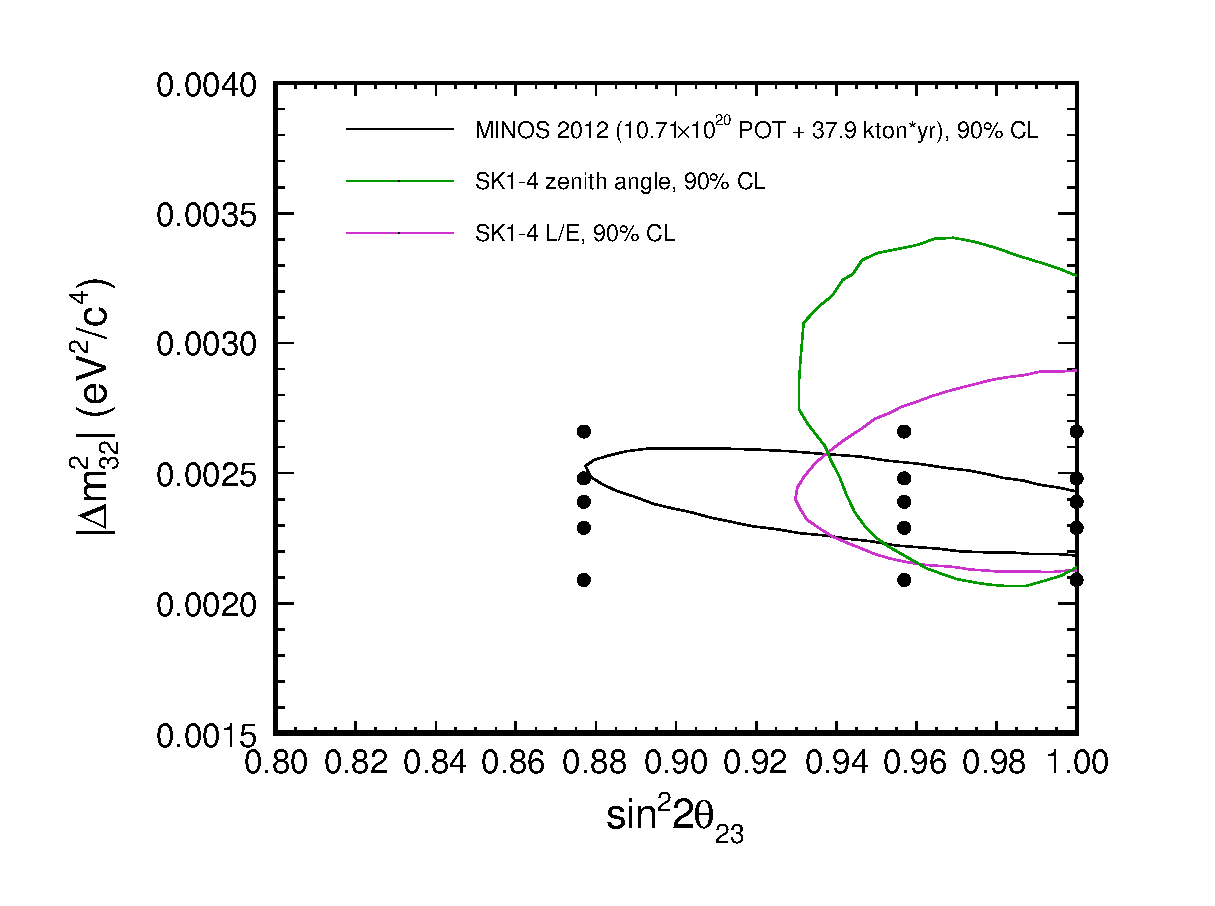
\includegraphics[width=35pc]{./images/sensitivities/sensitivity_study_points.eps}
\caption {
 True oscillation parameters points considered in our T2K sensitivity study.
 The grid was constructed using the 2012 MINOS best-fit $\Delta m_{32}^2$ value 
 and $\pm$1$\sigma$, $\pm$3$\sigma$ variations, and using 
 sin$^22\theta_{23}$ values
 of 1 (maximal), 0.957 (2012 MINOS best-fit value) and 0.877 (smallest value in the 2012 MINOS 90\% confidence region).
}
\label{fig:sensitivity_study_points}
\end{figure*}

An average $\chi^2$ surface was constructed as a function of sin$^22\theta_{23}$ and $\Delta m_{32}^2$ by averaging the 
$\chi^2$ surfaces obtained by `2+8' fits to 1K toy MC experiments. In each of these toy experiments, the systematic 
parameters were randomized and statistical fluctuations were included. The confidence contours were then drawn using 
the constant-$\Delta\chi^{2}$ method as described in Sec.\ \ref{sec:contour_construction_constdchi}.

%The $\Delta\chi^2$ surface was then constructed as
%$\Delta\chi^2$ = $\chi^2_{mean}$ - $min(\chi^2_{mean}$)

The results of the sensitivity study are shown in 
Figs. \ref{fig:sensitivity:2+8constdchisq:0.00209}-\ref{fig:sensitivity:2+8constdchisq:0.00266}.

%...........................................
%
%
\begin{figure*}[htb]
\begin{minipage}[t]{0.48\linewidth}
\center
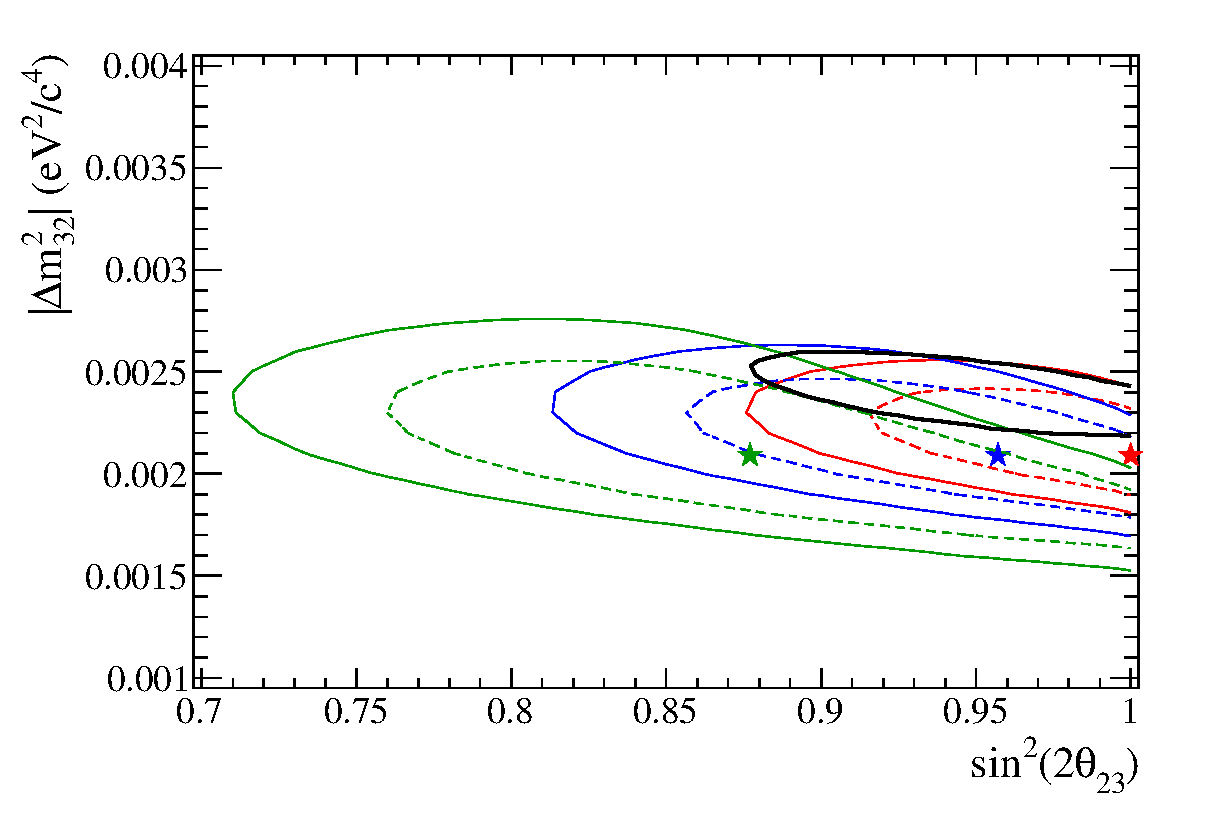
\includegraphics[width=18pc]{./images/sensitivities/2+8constdchisq/sensitivity_1}
\caption {
  T2K 68\% CL and 90\% CL sensitivity contours, for $3.010 \times 10^{20}$ POT, computed using the `2+8' fit.
  The input (sin$^22\theta_{23}$, $\Delta m_{32}^2$ (in $eV^{2}/c^{4}$)) points
  shown in red, blue and green are, respectively,
  (1.000, 0.00209), 
  (0.957, 0.00209), 
  (0.877, 0.00209).
  The 2012 MINOS 90\% CL region is shown in black.
}
\label{fig:sensitivity:2+8constdchisq:0.00209}
\end{minipage}
\hspace{0.06\linewidth}
\begin{minipage}[t]{0.48\linewidth}
\center
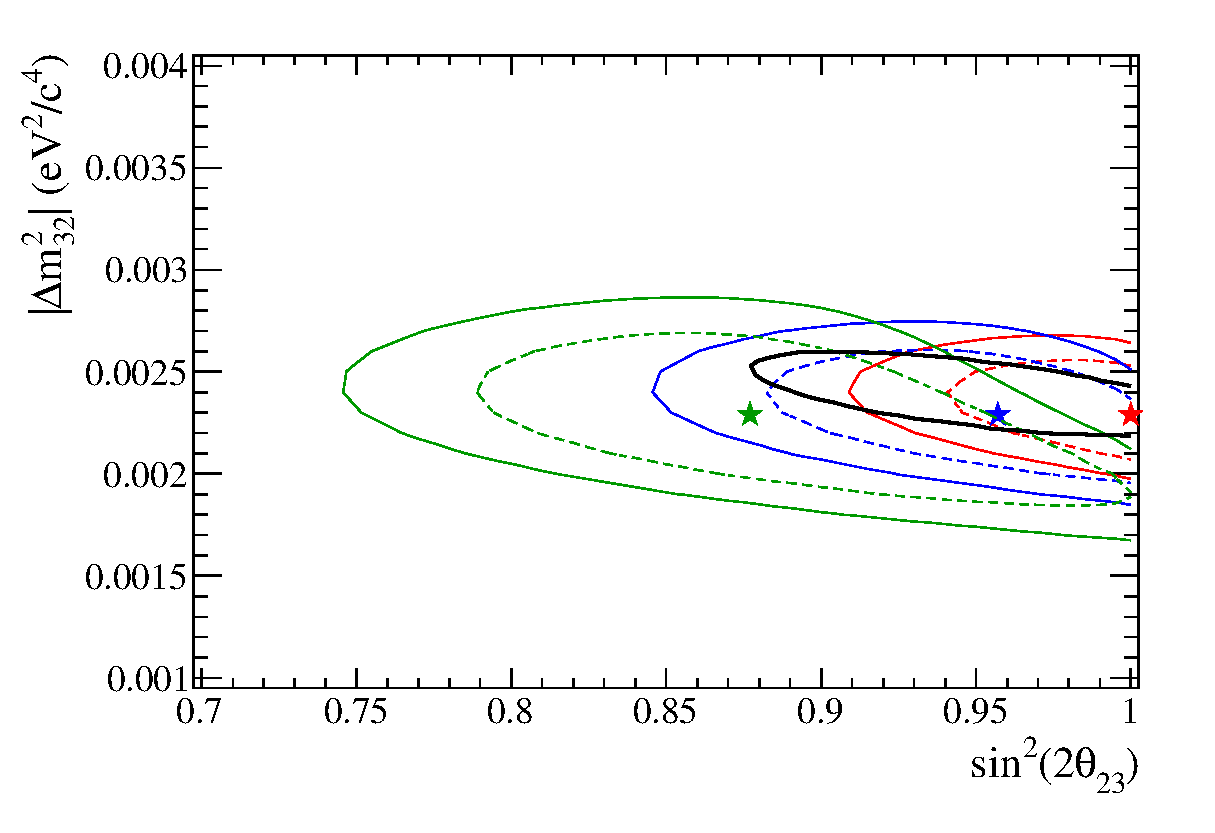
\includegraphics[width=18pc]{./images/sensitivities/2+8constdchisq/sensitivity_2}
\caption {
  T2K 68\% CL and 90\% CL sensitivity contours, for $3.010 \times 10^{20}$ POT, computed using the `2+8' fit.
  The input (sin$^22\theta_{23}$, $\Delta m_{32}^2$ (in $eV^{2}/c^{4}$)) points 
  shown in red, blue and green are, respectively,
  (1.000, 0.00229), 
  (0.957, 0.00229), 
  (0.877, 0.00229).
  The 2012 MINOS 90\% CL region is shown in black.
}
\label{fig:sensitivity:2+8constdchisq:0.00229}
\end{minipage}
\end{figure*}


\begin{figure*}[htb]
\begin{minipage}[t]{0.48\linewidth}
\center
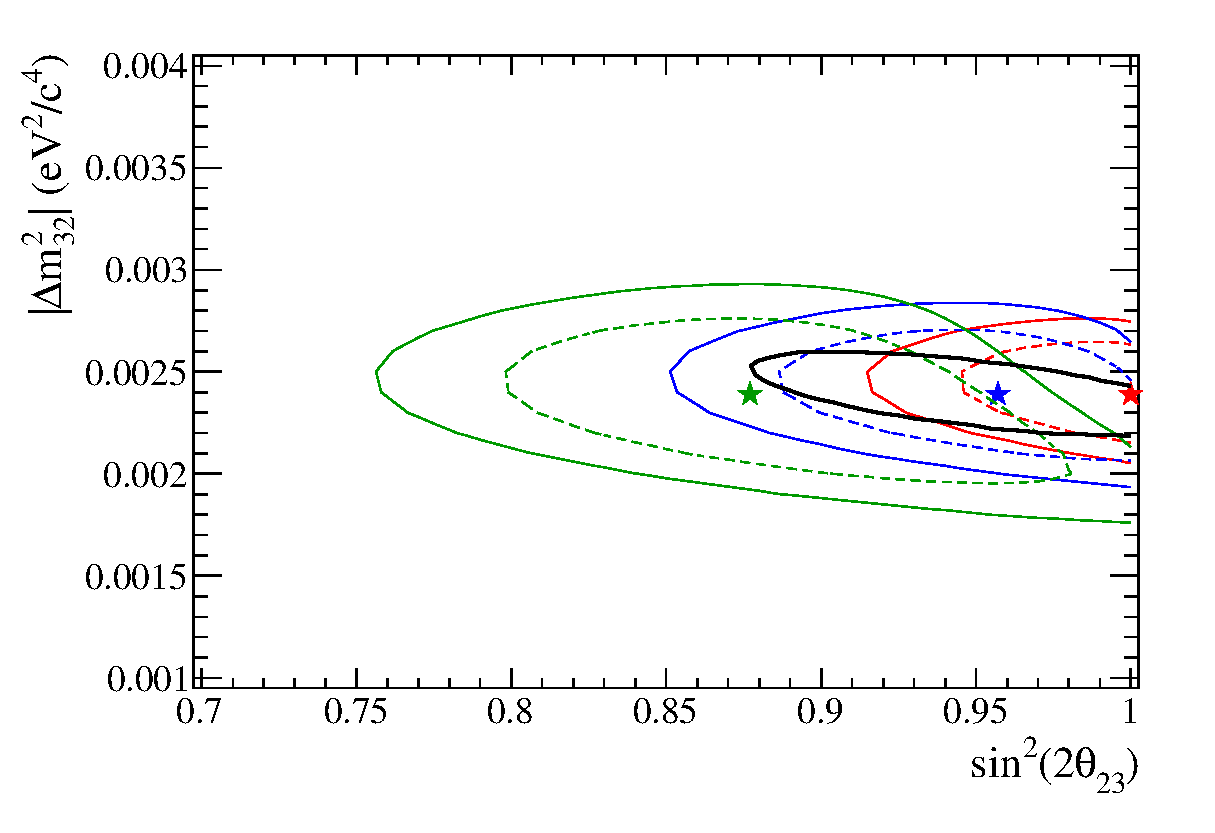
\includegraphics[width=18pc]{./images/sensitivities/2+8constdchisq/sensitivity_3}
\caption {
  T2K 68\% CL and 90\% CL sensitivity contours, for $3.010 \times 10^{20}$ POT, computed using the `2+8' fit.
  The input (sin$^22\theta_{23}$, $\Delta m_{32}^2$ (in $eV^{2}/c^{4}$)) points 
  shown in red, blue and green are, respectively,
  (1.000, 0.00239), 
  (0.957, 0.00239), 
  (0.877, 0.00239).
  The 2012 MINOS 90\% CL region is shown in black.
}
\label{fig:sensitivity:2+8constdchisq:0.00239}
\end{minipage}
\hspace{0.06\linewidth}
\begin{minipage}[t]{0.48\linewidth}
\center
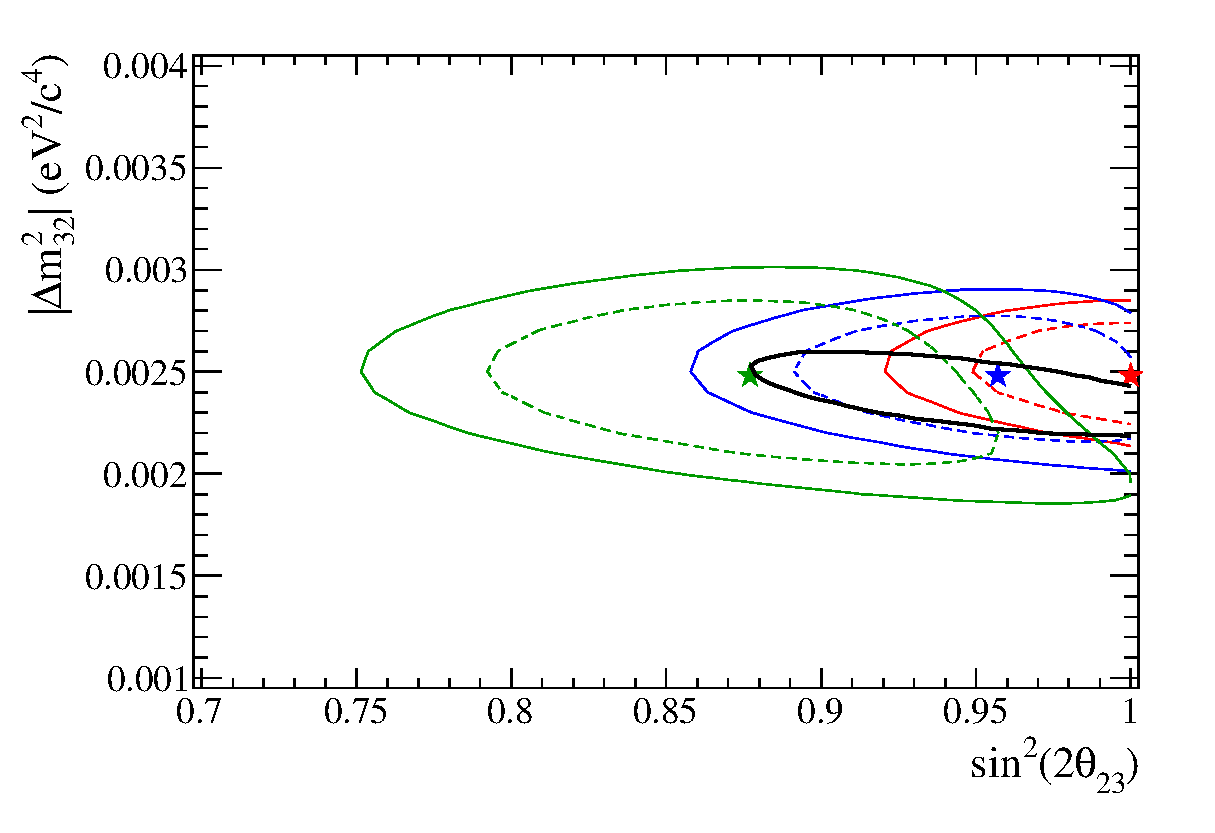
\includegraphics[width=18pc]{./images/sensitivities/2+8constdchisq/sensitivity_4}
\caption {
  T2K 68\% CL and 90\% CL sensitivity contours, for $3.010 \times 10^{20}$ POT, computed using the `2+8' fit.
  The input (sin$^22\theta_{23}$, $\Delta m_{32}^2$ (in $eV^{2}/c^{4}$)) points 
  shown in red, blue and green are, respectively,
  (1.000, 0.00248), 
  (0.957, 0.00248), 
  (0.877, 0.00248).
  The 2012 MINOS 90\% CL region is shown in black.
}
\label{fig:sensitivity:2+8constdchisq:0.00248}
\end{minipage}
\end{figure*}


\begin{figure*}[htb]
\begin{minipage}[t]{0.48\linewidth}
\center
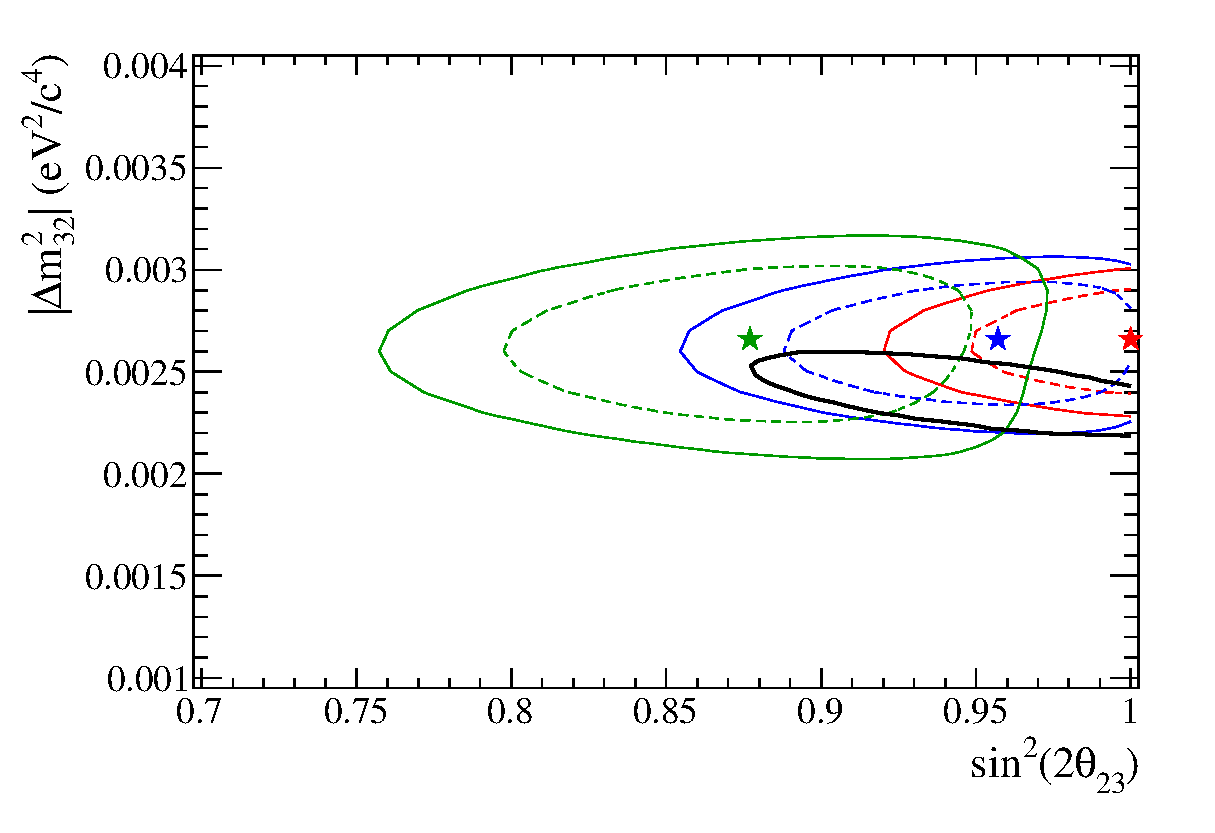
\includegraphics[width=18pc]{./images/sensitivities/2+8constdchisq/sensitivity_0}
\caption {
  T2K 68\% CL and 90\% CL sensitivity contours, for $3.010 \times 10^{20}$ POT, computed using the `2+8' fit.
  The input (sin$^22\theta_{23}$, $\Delta m_{32}^2$ (in $eV^{2}/c^{4}$)) points 
  shown in red, blue and green are, respectively,
  (1.000, 0.00266), 
  (0.957, 0.00266),  
  (0.877, 0.00266).
  The 2012 MINOS 90\% CL region is also shown in black.
}
\label{fig:sensitivity:2+8constdchisq:0.00266}
\end{minipage}
\end{figure*}
